\documentclass[12pt,a4paper]{article}
\usepackage[UTF8]{ctex}     %先引入ctex
\usepackage[utf8]{inputenc} %再引入inputenc
\usepackage{graphicx}
% \usepackage{lazylatex}
% \tcbuselibrary{documentation}
\usepackage{amsmath}
\usepackage{amssymb}
\usepackage{bookmark}
\usepackage{enumerate}
\usepackage{geometry}
\usepackage{tikz}
\usepackage{forest}
\usepackage{float}
\usetikzlibrary{automata,positioning}

\graphicspath{{img/}}
% 边距
\geometry{left=2.0cm,right=2.0cm,top=1.0cm,bottom=3.0cm}
% 大题
\newenvironment{problems}{\begin{list}{}{\renewcommand{\makelabel}[1]{\textbf{##1}\hfil}}}{\end{list}}
% 小题
\newenvironment{steps}{\begin{list}{}{\renewcommand{\makelabel}[1]{##1)\hfil}}}{\end{list}}
% 答
\providecommand{\ans}{\textbf{答}:~}
% 解
\providecommand{\sol}{\textbf{解}.~}

\begin{document}
\title{\normalsize \underline{编译原理(A)}\\\LARGE第 4 次作业}
\author{Log Creative }
\date{\today}
\maketitle

\begin{problems}
    \item[1] 为下列正则表达式或语言设计一个DFA或NFA
    \begin{steps}
        \item[1] $a(a|b)^*a$
        
        \ans 
        \begin{figure}[H]
            \usetikzlibrary {automata,positioning}
\begin{tikzpicture}[shorten >=1pt,node distance=2cm,on grid,auto]
	\node[state,initial] (0) {$0$};
	\node[state,right of=0] (1) {1};
	\node[state,right of=1] (2) {2};
	\node[state,above right of=2] (3) {3};
	\node[state,right of=3] (5) {5};
	\node[state,below right of=2] (4) {4};
	\node[state,right of=4] (6) {6};
	\node[state,below right of=5] (7) {7};
	\node[state,right of=7] (8) {8};
	\node[state,right of=8,accepting] (9) {9};
	\path[->] (0) edge node {$a$} (1)
		(1) edge node {$\epsilon$} (2)
		(2) edge node {$\epsilon$} (3)
		(2) edge node {$\epsilon$} (4)
		(3) edge node {$a$} (5)
		(4) edge node {$b$} (6)
		(5) edge node {$\epsilon$} (7)
		(6) edge node {$\epsilon$} (7)
		(7) edge node {$\epsilon$} (8)
		(7) edge [out=90,in=90,looseness=1.5] node {$\epsilon$} (2)
		(1) edge [out=-60,in=-120] node {$\epsilon$} (8)
		(8) edge node {$a$} (9);
\end{tikzpicture}

        \end{figure}
        
        \item[2] $((\epsilon|a)b^*)^*$
        
        \ans 
        \begin{figure}[H]
            \usetikzlibrary {automata,positioning}
\begin{tikzpicture}[shorten >=1pt,node distance=2cm,on grid,auto]
	\node[initial,state] (0) {0};
	\node[state,right of=0] (1) {1};
	\node[state,below right of=1] (2) {2};
	\node[state,right of=2] (3) {3};
	\node[state, above right of=3] (4) {4};
	\node[state,right of=4] (5) {5};
	\node[state,right of=5] (6) {6};
	\node[state,right of=6] (7) {7};
	\node[accepting,state,right of=7] (8) {8};
	\draw (0) edge[->] node {$\epsilon$} (1)
		%(1) edge[->] node {$\epsilon$} (2)
		(1) edge[->] node {$\epsilon$} (2)
		(2) edge[->] node {$a$} (3)
		(1) edge[->] node {$\epsilon$} (4)
		(3) edge[->] node {$\epsilon$} (4)
		(4) edge[->] node {$\epsilon$} (5)
		(5) edge[->] node {$b$} (6)
		(6) edge[->] node {$\epsilon$} (7)
		(7) edge[->] node {$\epsilon$} (8)
		(6) edge[->,in=90,out=90] node {$\epsilon$} (5)
		(4) edge[->,in=-120,out=-60] node {$\epsilon$} (7)
		(7) edge[->,in=45,out=135] node {$\epsilon$} (1)
		(0) edge[->,in=-140,out=-40] node {$\epsilon$} (8);
\end{tikzpicture}

        \end{figure}
        
        \item[3] $(a|b)^*a(a|b)(a|b)$
        
        \ans
        \begin{figure}[H]
            \usetikzlibrary {automata,positioning}
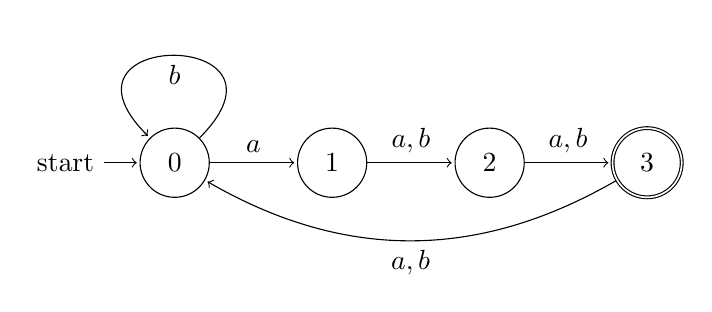
\begin{tikzpicture}[shorten >=1pt,node distance=2cm,on grid,auto]
	\node[initial,state] (0) {0};
	\node[state,right of=0] (1) {1};
	\node[state,right of=1] (2) {2};
	\node[accepting,state,right of=2] (3) {3};
	\path (0) edge[->] node {$a$} (1)
		 (1) edge[->] node {$a,b$} (2)
		 (2) edge[->] node {$a,b$} (3)
		 (0) edge [loop] node {$b$} (0)
		 (3) edge[->,out=-150,in=-30] node {$a,b$} (0) ;
\end{tikzpicture}

        \end{figure}
        \item[4] $a^*ba^*ba^*ba^*$
        
        \ans
        \begin{figure}[H]
            \usetikzlibrary {automata,positioning}
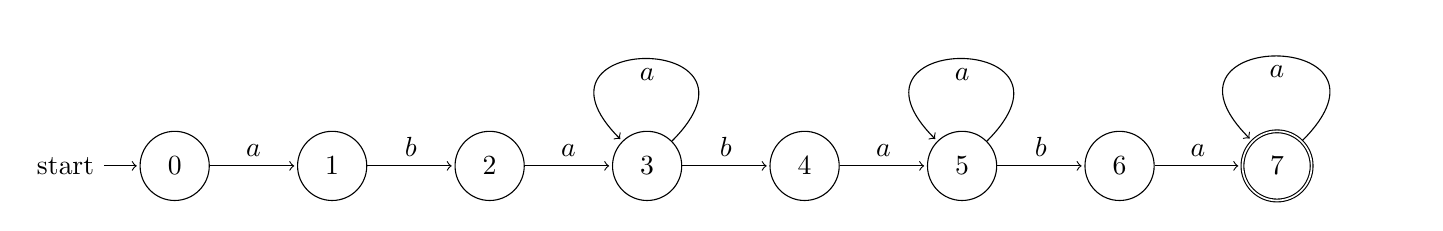
\begin{tikzpicture}[shorten >=1pt,node distance=2cm,on grid,auto]
	\node[initial,state] (0) {0};
	\node[state,right of=0] (1) {1};
	\node[state,right of=1] (2) {2};
	\node[state,right of=2] (3) {3};
	\node[state,right of=3] (4) {4};
	\node[state,right of=4] (5) {5};
	\node[state,right of=5] (6) {6};
	\node[accepting,state,right of=6] (7) {7};
	\path (0) edge[->] node {$a$} (1)
		 (1) edge[->] node {$b$} (2)
		 (2) edge[->] node {$a$} (3)
		 (3) edge[->] node {$b$} (4)
		 (4) edge[->] node {$a$} (5)
		 (5) edge[->] node {$b$} (6)
		 (6) edge[->] node {$a$} (7)
		 (3) edge[loop] node {$a$} (3)
		 (5) edge[loop] node {$a$} (5)
		 (7) edge[loop] node {$a$} (7);
\end{tikzpicture}

        \end{figure}
        \item[5] 所有由偶数个a和奇数个b构成的串
        
        \ans
        \begin{figure}[H]
            \usetikzlibrary {automata,positioning}
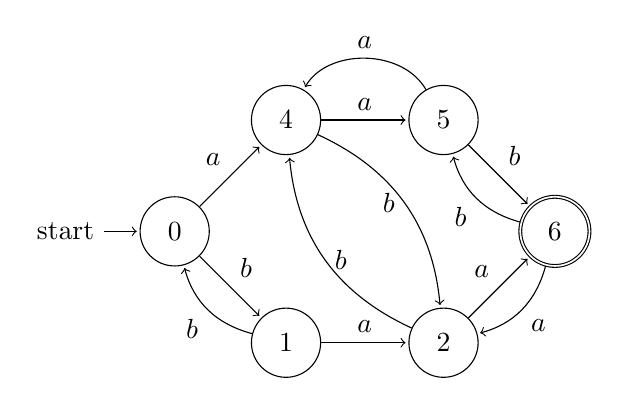
\begin{tikzpicture}[shorten >=1pt,node distance=2cm,on grid,auto]
	\node[initial,state] (0) {0};
	\node[state,below right of=0] (1) {1};
	\node[state,right of=1] (2) {2};
	\node[accepting,state,above right of=2] (6) {6};
	\node[state,above right of=0] (4) {4};
	\node[state,right of=4] (5) {5};
	\path (0) edge [->] node {$b$} (1)
		(1) edge[->] node {$a$} (2)
		(2) edge[->] node {$a$} (6)
		(0) edge[->] node {$a$} (4)
		(4) edge[->] node {$a$} (5)
		(5) edge[->] node {$b$} (6)
		(5) edge[->,out=120,in=60] node[above]  {$a$} (4)
		(6) edge[->,bend left] node {$b$} (5)
		(1) edge[->,bend left] node {$b$} (0)
		(6) edge[->,bend left] node {$a$} (2)
		(4) edge[->,bend left] node[left] {$b$} (2)
		(2) edge[->,bend left] node[right] {$b$} (4);
\end{tikzpicture}

        \end{figure}
    \end{steps} 
    \item[2] 给出下列两个NFA的转换表:
    \begin{steps}
        \item[1]
        
         \usetikzlibrary{graphs,rdf}
\tikzset{
dfa/.style = { semithick, > = To [sep] },
nfa/.style = { semithick, > = To [sep] },
state/.style = { circle, draw, minimum size = 1cm },
final/.style = { double },
initial/.style = { draw = red }, % to keep things simple
transition/.style = { edge label = {$#1$} }
}
\begin{tikzpicture}[nfa]
	\graph [math nodes, grow right = 1.5cm]{
		start ->
		0 [state,initial] -> [transition = {a,b}, loop below]
		0 -> [transition=a]
		1 [state] -> [transition = {a,b}, loop below]
		1 -> [transition=a]
		2[state] -> [transition = {a,b}, loop below]
		2 -> [transition=b]
		3[state, final];
		2 -> [transition=\epsilon,out=130,in=50]
		0;
	};
\end{tikzpicture}


         \begin{tabular}{c|ccc}
            状态 & $a$ & $b$ & $\epsilon$\\
             \hline
            0 & \{0,1\} & \{0\} & $\varnothing$\\
            1 & \{1,2\} & \{1\} & $\varnothing$ \\
            2 & \{2\} & \{2,3\} & \{0\} \\
            3 & $\varnothing$ & $\varnothing$ & $\varnothing$
         \end{tabular}
        \item[2] 
        
         \usetikzlibrary {automata,positioning}
\begin{tikzpicture}[shorten >=1pt,node distance=2cm,on grid,auto]
	\node[initial,state] (0) {0};
	\node[state,right of=0] (1) {1};
	\node[state,above right of=1] (2) {2};
    \node[state,below right of=1] (3) {3};
    \node[state,right of=2] (4) {4};
    \node[state,right of=4] (5) {5};
    \node[state,right of=5] (6) {6};
    \node[state,right of=3] (7) {7};
    \node[state,right of=7] (8) {8};
    \node[state,right of=8] (9) {9};
    \node[state,below right of=6] (10) {10};
    \node[accepting,state,right of=10] (11) {11};
    \path (0) edge[->] node {$\epsilon$} (1)
        (1) edge[->] node {$\epsilon$} (2)
        (1) edge[->] node {$\epsilon$} (3)
        (2) edge[->] node {$\epsilon$} (4)
        (3) edge[->] node {$\epsilon$} (7)
        (4) edge[->] node {$a$} (5)
        (7) edge[->] node {$b$} (8)
        (5) edge[->] node {$\epsilon$} (6)
        (8) edge[->] node {$\epsilon$} (9)
        (6) edge[->] node {$\epsilon$} (10)
        (9) edge[->] node {$\epsilon$} (10)
        (10) edge[->] node {$\epsilon$} (11)
        (0) edge[->,out=-90,in=-90] node {$\epsilon$} (11)
        (10) edge[->,out=90,in=90,above] node {$\epsilon$} (1)
        (2) edge[->,out=30,in=150] node {$\epsilon$} (6)
        (3) edge[->,out=-30,in=-150] node {$\epsilon$} (9)
        (5) edge[->,out=-90,in=-90,above] node {$\epsilon$} (4)
        (8) edge[->,out=90,in=90,below] node {$\epsilon$} (7);
	
\end{tikzpicture}


         \begin{tabular}{c|ccc}
            状态 & $a$ & $b$ & $\epsilon$\\
             \hline
            0 & \{1\} & $\varnothing$ & \{3\}\\
            1 & $\varnothing$ & \{2\} & \{0\} \\
            2 & $\varnothing$ & \{3\} & \{1\} \\
            3 & $\varnothing$ & $\varnothing$ & \{0\}
         \end{tabular}
    \end{steps} 
\end{problems}


\end{document}
